\section{Ejercicio 3}

\subsection{Ejemplo de sharding en Mongo}

Seguimos las sugerencias del enunciado y analizamos los efectos de usar sharding simple o hasheado en una base de datos en la que insertamos iterativamente tandas de a 20000 registros, para un total de 25 tandas. A continuaci'on mostramos los gr'aficos de carga de los shards a lo largo de las iteraciones:

\begin{figure}[H]
	\begin{center}
		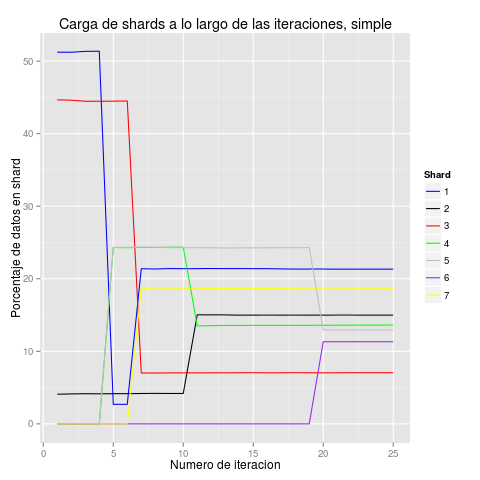
\includegraphics[scale=0.6]{imagenes/siete_shards_simple.png}
	\end{center}
\end{figure}

\begin{figure}[H]
	\begin{center}
		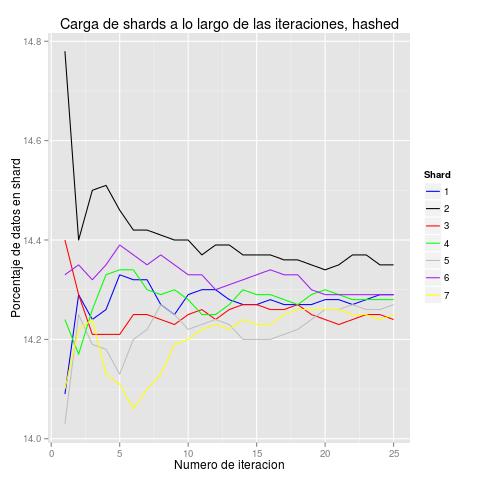
\includegraphics[scale=0.6]{imagenes/siete_shards_hashed.png}
	\end{center}
\end{figure}

Recordemos que el atributo usado de clave para los shards es el codigo postal, que es un entero de hasta 6 d'igitos. Como podemos apreciar, cuando hacemos sharding hasheando el codigo postal, la distribuci'on de los datos a lo largo de los shards tiende a estar bien balanceada. Por el contrario, si no se hashea el codigo postal, mongo empieza cargando fuertemente dos shards, y luego empiezan a tener mas participacion otros. Esto se debe a que la forma de determinar qu'e documentos van a qu'e shards cuando la clave no se hashea est'a determinado por rangos del c'odigo postal, que mongo no conoce a priori y debe ir estimando. Una vez que la cantidad de datos crece, mongo puede inferir que la distribuci'on en uniforme entre cero y un millon y la carga se empieza a equilibrar al darle rangos equitativos de responsabilidad a cada shard. Pero al principio, la distribuci'on es extremadamente dispareja.

\subsection{Caracter'isticas de un buen atributo para sharding}

Para que un atributo sea un buen candidato para aplicar la t'ecnica de sharding, debe ser tal que al particionar los datos por ese atributo, las clases que se formen sean de tama\~nos similares. Esto permite que la carga sobre los shards est'e bien distribu'ida, no s'olo en t'erminos del vol'umen de cada shard, sino tambi'en en el sentido de que los accesos y escrituras sean uniformes. Bajo estas condiciones obtendremos una mejor performance de I/O. Espec'ificamente, la latencia y el tiempo de respuesta de los mismos ser'an bajos, gracias a que evitamos cuellos de botella.

Para ilustrar esto, pensemos en un mal ejemplo de sharding. Consideremos una base de datos que contenga los datos de los alumnos del Departamento de Computaci'on de la facultad. Si hacemos sharding sobre el atributo \emph{g'enero}, tendremos dos shards completamente asim'etricos en su tama\~no. Claramente, la enorme mayor'ia de los accesos ser'an sobre el shard de alumnos de sexo masculino, lo cual tiene un obvio impacto en la performance.

Vale la pena mencionar que el sharding puede ser de utilidad no s'olo para asegurar balanceo de carga. En ciertos sistemas, son habituales las consultas que necesitan revisar 'unicamente un subconjunto de todo el universo de elementos. En estos casos, es 'util hacer sharding de modo tal de que uno de estos subconjuntos que nos interesan est'en separados en shards. Tomemos como ejemplo un base de datos de una red social, en la cual se hace sharding por el pa'is de residencia de las personas. En este caso, podremos optimizar la consulta \textit{amigos de una persona}, puesto que, en general, la mayor parte de los amigos de una persona est'an geogr'aficamente cerca.

\subsection{Ejemplos de sharding}

Algunos ejemplos de una buena elecci'on de un atributo para hacer sharding son los siguientes:

\begin{enumerate}
	\item Sharding por atributo \emph{g'enero} en una base de datos del padr'on electoral de un pa'is.
	\item Sharding por atributo \emph{pa'is de residencia} en una base de datos de personas de una red social.
	\item Sharding por atributo \emph{a\~no de nacimiento} en una base de datos de personas nacidas durante cierto per'iodo de tiempo, fijo. Por ejemplo, durante la dictadura de 1976.
\end{enumerate}

Se puede ver que en los tres casos, la proporci'on de los grupos en los que clasificamos es aproximadamente la misma, y que, a priori, no deber'ia haber ninguna tendencia de acceso a un shard en particular.

Una alternativa siempre 'util es hacer sharding utilizando hashing. Esto significa tomar un atributo cuya distribuci'on sea m'as o menos uniforme (por ejemplo, un atributo identificatorio o un n'umero de tel'efono), y shardear utilizando el hasheo del atributo. 